
%(BEGIN_QUESTION)
% Copyright 2006, Tony R. Kuphaldt, released under the Creative Commons Attribution License (v 1.0)
% This means you may do almost anything with this work of mine, so long as you give me proper credit

Some electronic controllers provide the option of a {\it time-proportioning} output instead of the customary {\it current-proportioning} output.  With the time-proportioning output, the two output terminals of the controller connect (internally) to a relay contact or transistor, capable only of turning an electrical load fully on and fully off:

$$\includegraphics[width=15.5cm]{i01487x01.eps}$$

Time-proportional control is most often used when the final control element is an electric heater.  Explain how time-proportional control works to maintain a process variable at setpoint while only being able to turn a heater on and off (and not in-between).

\underbar{file i01487}
%(END_QUESTION)





%(BEGIN_ANSWER)

The controller outputs a {\it Pulse-Width Modulated} signal, the duty cycle of the on/off cycling modulating energy input to the process through the heating element.

%(END_ANSWER)





%(BEGIN_NOTES)


%INDEX% Control, proportional: time-proportioning output

%(END_NOTES)


